% Typeset by:
%  Will Crawford (wacrawfo@ucsc.edu)

\documentclass[12pt,article]{memoir}
% \usepackage{amsmath}
\usepackage{graphicx}
\graphicspath{{./img/}}
\pagestyle{empty} % no headers or footers

\title{S.C.O.R.E Report for\\ MyCourses \\ A Course Scheduling System \\ UCSC Team}
\author{Ben Ross \texttt{(benr22@gmail.com)} \\
	\and Erik Steggall \texttt{(eqstegall@gmail.com)}\\
	\and Justin Lazaro \texttt{(jlazaro@ucsc.edu)}\\
	\and Sabba Petri \texttt{(sabbap@gmail.com)}\\
	\and Will Crawford \texttt{(wacrawfo@ucsc.edu)}}
\date{}
% \setcounter{secnumdepth}{-1}

\begin{document}

\maketitle

\chapter{Development Process} % Will

\chapter{Requirements: Problem Statement} % Justin
\chapter{Requirements: Specification} % Sabba
This section is designed to provide an overview of S.C.O.R.E. Scheduling based upon the requirements above. Within this section, one will understand the power behind the technology used for this system: the web server technology and the algorithm used to schedule the classes. To begin, the web server for the S.C.O.R.E. Scheduling system is Django, strictly because of its ability to ease the creation of database-driven websites. It provides an abstracted framework for dynamic websites that is easy to learn and easy to integrate. The available components also will help us throughout this design process, such as the clever template system interfacing with the user interface. Django is written in Python, which is the language of choice for this project, as well as the language of our algorithm.

When deciding upon an algorithm, we needed to decide whether to go with a constraint-based solver, or to design an algorithm in-house to fulfill out needs. Because the scheduling problem is an NP-Hard problem, by using a constraint-based solver, it would ease the programming end of the algorithm team; however, learning to use a constraint-based solver would require more time to learn. On the other side to this decision, designing an algorithm in-house would provide full control of the algorithm in how we decide to integrate it with the web server framework.

Looking at figure three, the class diagram depicts an overall outlook of our in-house algorithm, of which will be the heart and engine of our Scheduling system. This class diagram shows the relationship between the configuration Python file with the different database attributes, such as professor, course, room, schedule, and course class. The configuration class is the primary driver that weaves all the user groups and database attributes together to function as a single entity.  

% See http://en.wikibooks.org/wiki/LaTeX/Importing_Graphics#Images_as_Figures
\begin{figure}[htb]
%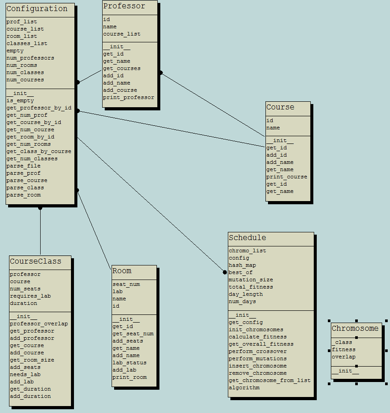
\includegraphics{classDiagram.jpg}
\caption{Class Diagram of Algorithm}
\end{figure}

Once one understands the algorithm above, then it can then be applied to the multiple use cases that it will be serving for. The interaction diagrams below contain every interaction of each user: student, lecturer, program manager, and program administrator. Each diagram details a pictorial representation of the user’s interaction with the system, such as the HTML website, the Django engine, the database that’s handled, or the algorithm itself.  In all these diagrams, the HTML portal, or front-end website, is an input/output object wherein users will input items and receive output from Django. From behind the front-end website, Django serves as a control object that handles all aspects of user, algorithm, and database interactions. The database itself is an entity that stores information from user input processed by Django, and it also provides output to the user. Lastly, the algorithm is a control entity that manipulates the database courses, but all functionality of the algorithm remains hidden from the entire system. 

\begin{figure}[htb]
%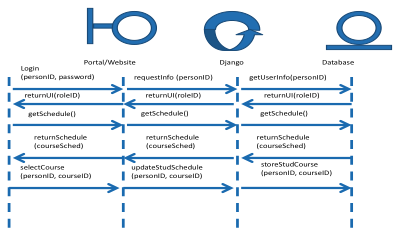
\includegraphics{studentID.jpg}
\caption{Student interaction diagram}
\end{figure}

\begin{enumerate}
\item The student will login with their ID and password on the portal. Django will read the ID and password and match it with the database. 
\item Once the database confirms user, the database will return the correct UI for the student.
\item The student will want to get the schedule of classes to sign up for and “makes a request” to Django and the database to display the available courses. By “making a request”, this is done invisible to the user and the user will simply click on the courses tab. It will open automatically for the user. 
\item The student can now select courses and store them into their profile on the database. 
\end{enumerate}

\begin{figure}[htb]
%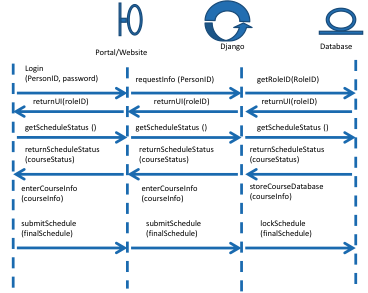
\includegraphics{programAdminID.jpg}
\caption{Program Admin enters courses interaction diagram}
\end{figure}

\begin{enumerate}
\item The program administrator will login with their ID and password on the portal. Django will read the ID and password and match it with the database. 
\item Once the database confirms user, the database will return the correct UI for the program administrator.
\item The program administrator will want to know the status of the schedule, to see if it is finished or not, and will make a request to both Django and the database to find out the status. 
\item The database will return the status. 
\item The program administrator will begin filling out course information through a courseInfo object that will contain various data about a given course.
\item When the program administrator feels done, they can choose to submit the course and lock the course in the database. 
\end{enumerate}

\begin{figure}[htb]
%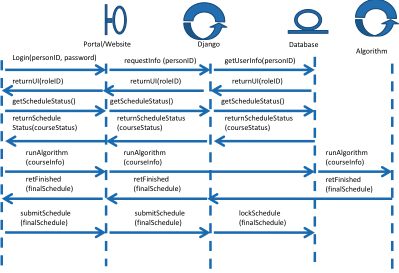
\includegraphics{programAdminID2.jpg}
\caption{Program Administrator runs algorithm interaction diagram}
\end{figure}

\begin{enumerate}
\item The program administrator will login with their ID and password on the portal. Django will read the ID and password and match it with the database. 
\item Once the database confirms user, the database will return the correct UI for the program administrator.
\item The program administrator will want to know the status of the schedule, to see if it is finished or not, and will make a request to both Django and the database to find out the status. 
\item The database will return the status to see if the program manager has completed the schedule. 
\item If the schedule is complete, the program administrator will run the algorithm that will be passed through Django and straight into the algorithm engine.
\item When the engine has completed, it will return a message that it is complete to the HTML website. 
\item Once the program administrator reviews the schedule, the program administrator can submit and lock the schedule and provide it to students
\end{enumerate}

\begin{figure}[htb]
%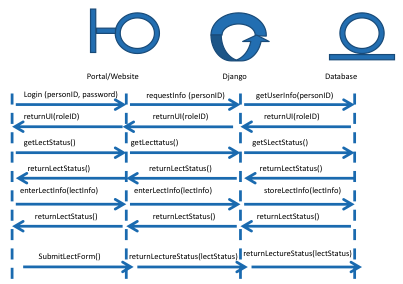
\includegraphics{lecturerID.jpg}
\caption{Lecturer interaction diagram}
\end{figure}

\begin{enumerate}
\item The lecturer will login with their ID and password on the portal. Django will read the ID and password, and match it with the database. 
\item Once the database confirms user, the database will return the correct UI for the lecturer.
\item The lecturer will want to find out the constraint form has been completed. Upon logging in, Django will send a message on the status of his constraint form, based upon a status in the database.
\item The lecturer will fill out the constraint form and store it in the database.
\item Upon storing it in the database, the lecture status will be updated and confirmed. 
\item The lecturer can now formally submit his constraints form to the database. 
\end{enumerate}

\begin{figure}[htb]
%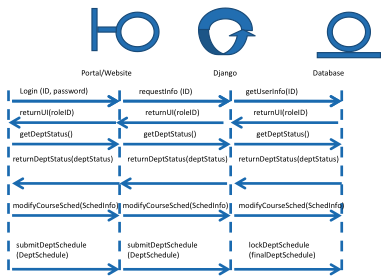
\includegraphics{programManagerID.jpg}
\caption{Program Manager interaction diagram}
\end{figure}

\begin{enumerate}
\item The program manager will login with their ID and password on the portal. Django will read the ID and password and match it with the database. 
\item Once the database confirms user, the database will return the correct UI for the program manager.
\item Upon logging in, Django will automatically send a request to find out the department status of the courses. 
\item If the status is not yet been completed, it will send a message to the program manager.
\item The program manager can modify the courses that was made available from the program administrator and placed in the database. 
\item Upon modifying the courses and the course info, the program manager can confirm and submit the finalized course. 
\end{enumerate}


\chapter{Architectural Design} % Erik
Our architecture is broken into three main categories:
\begin{enumerate}
\item User interface or UI (The front end)
\item Django (The back end)
\item The algorithm (The engine)
\end{enumerate}

\section{The User Interface}
There are four different user interfaces, each is assigned to one of the four roles that a user could be: Program administrator, program manager, lecturer, student. The students UI is the most complex and offers the most customization.

The program administrators user interface is fairly simple, they are given fields such as courses, rooms, and professors to fill out, once they fill out the fields to the proper specifications for the quarter then they have an option to run the algorithm. The algorithm will run, and then post up the results back to the program manager.

The program manager's interface will hold all of the courses and lecturers for their department. The program manager will have the option of selecting the lecturers and courses that they want to be active for the quarter.

The lecturer will have an interface that will hold the courses that they can teach and the current courses that they are teaching. 
The student will have a customizable interface which will hold their past, present and future schedules. It will also have other widgets that they will be able to add to their profile.
\section{Django}
Django connects the user interface, the database and the algorithm. Django manages the user interface by handling the user requests and providing the appropriate response. In the case of the algorithm it takes the request from the program administrator to run the algorithm and creates a request object and sends it through multiple middlewares (Python functions). Django then checks the URLs to decide which function it must send the request object to. The function in this case is the algorithm, which takes the information stored in the program administrators database and runs. The output of the algorithm is placed into a second database and the request object is sent back up through the middleware in the reverse order of the way it came in. The second database is then displayed to the program administrator.

\section{The Algorithm}

\chapter{Project Plan} % Justin
\chapter{Management Plan} % Erik and Will
\chapter{Implementation} % Ben

Implementation of the MyCourses scheduling system was a multifaceted problem. The overall system was broken down into four main parts to implement: Web Interface, Database, Algorithm, and Security. Our implementation strategy was to find the best way to implement the parts separately, and then collectively integrate them together. This would allow us to selectively work on each part of the combined system separately.

The implementation of the Web Interface is done in HTML5, with a Django Server backend. HTML5 was selected over previous versions of the markup language because it allows development with less JavaScript and Flash. Even though these technologies are very popular on the Internet, staying away from them allows us to increase the browser compatibility of our system. As newer browsers are released, HTML5 support increases, which permits us to use newer features of the language to add newer features to the system as the client desires. 

The Django Server backend was selected for a few reasons. Django is a free Web Server backend that allows for easy control of databases, as well as Pythonic ways to display information on varying web pages. This allows us to integrate the algorithm with the database seamlessly. This was to be a major problem facing our system, but was quickly alleviated earlier in the process. Django uses forms and templates to display information from the database to web pages and this allows us to create a few templates for each of the authentication levels, all of which are able to display information directly from the database with no SQL queries. Because Django performs the CRUD on the database, Python queries are performed with great speed, letting pages to load quicker.

The Algorithm went through three different implementations before the best implementation was selected. The first implementation was a slow Algorithm designed by one of the team members. It was very inefficient, but allowed the program administrator complete history of the courses that were scheduled at a given time, in a given room. This allowed for easier manual edits of the proposed schedule. The second implementation was using a FLOSS constraint-solver Minion. This solution was very fast, but needed a complicated script to translate from the database to the solver and back again. The third implementation was a scheduling algorithm using a genetic Algorithm. This Algorithm was based off of a freeware genetic algorithm scheduler. The Algorithm was written in Python, allowing it to be fast and easily modifiable. The genetic Algorithm was selected as the best implementation solution, because it allowed seamless integration with the database, and it proves incredibly fast, even for larger solutions.

Security for our system was not something that came up in our initial discussions of the system. However, security is one of the most important aspects of a web application. Also, universities generally have lots of sensitive data displayed on similar applications and thus, security needs to be paramount. The security system we designed into our system also integrates with the privacy settings for the application. HTTPS is used instead of the HTTP; this allows all traffic coming to and from the system to be encrypted. This is a step above popular web applications like Facebook, and Myspace, providing students, faculty members, and administrators peace of mind, knowing their traffic will be very difficult to decrypt. Our second important security feature is passwords. Our minimum password length is 8, with a minimum of one capital letter, one symbol, and one letter. This allows users increased security from brute force password attacks. Another security feature involving passwords is similar to what some banks do. We assign each user a sitekey, which is a random picture out of 50. The user is then requested to name the sitekey. When the user enters their password, if an incorrect sitekey is displayed, the user is made aware of an attempt to compromise their information. 

The other security features deal with the privacy of the user once they are in the system. These features are designed for the student role only. The integration of Facebook with our system provided another way for our system to lose security. When the student first logs into the system, a tutorial walks them through setting up their account and linking it with their Facebook. The student has the option to turn off sharing of information during this setup, as well as, anytime through the account settings page. This feature gives permission to students for complete access as to what information they share through our system, and through Facebook. Allowing students this control will decrease the chances of a student sharing more information than they previously wanted to.

\chapter{Validation and Verification} % Ben and Erik
Our test framework for our implementation has two forms. Testing for the algorithm and testing for the web UI. The testing for the algorithm is done by scripts, and the web UI testing is done through a software suite.

The algorithm was first tested by running the algorithm and then manually checking the output. The output was checked to see if the proposed schedule was a valid schedule and to see if all of the constraints were met. This became very tedious for large class schedules, so a script was written that validates the output based on the constraints given in the database. This allowed large testing to be completed much faster.

The web UI testing is done using a framework called Selenium. This open source tool allows automatic testing of the web UI. Two methods were used for writing tests for the web UI. Selenium has an IDE that allows you to record an interaction with the web UI and
run that recording as a test. This was done for basic actions, such as logging in and out. The other way are python scripts that use Seleniums built in libraries to interact with the web interface. This allows the tester to check for output on a given page and to
perform more complex actions. This was done for advanced actions, such as signing up for classes, or adding students to the database.
\chapter{Outcomes and Lessons Learned} % All

\end{document}